\documentclass{article}
\usepackage[margin=0.9in]{geometry}
\usepackage{mathtools}
\usepackage{hyperref}
\renewcommand{\baselinestretch}{1.2}

\usepackage{float}
%\usepackage{wrapfig} % Allows in-line images such as the example fish picture
\usepackage[pdftex]{graphicx} 
\graphicspath{{scrachPlot/}} % declare the path(s) where your graphic files
\author{Jiang Han, Haitao Liu, Chong Zhou}
\begin{document}
\title{Data Visualization Final Project Process book} 
\date{November 6, 2016}
\maketitle

\section{Overview and Motivation}
Education is a key factor in affecting people career and achievement in the later-on life. So it's interesting to understand how the students' background and personal effort impact the learning process. We have a real-world dataset that include such factors, such as student grades, demographic, social and school related features. For the learning measurement, the dataset consists of the grade of Math and Portuguese, where are the targets that we could predict from the student background, personal efforts and other social and school related features. The reason that we choose this dataset is that educational data mining is very interesting by exploring the factors that contributes to the success of learning. If such factors are well understand and discovered, we can help the students learn more effective and efficient. Another reason is from our personal experiences, Both learning a foreign language and learning the math needs some ``talents''. But the talent needed for language and math seems different, since math and language are processed in different area of our brain . Based on the above motivation, we would like to explore the relation between students' background and their grades in math and Portuguese and also to verify our assumption that the ``talents'' for math and Portuguese are different.

\section{Relate Work}
Paulo Cortez and Alice Silva (2008) predicated the student performance by applying Decision Trees, Random Forest, Neural Networks and Support Vector Machines algorithm. And also three input selections (e.g. with and without previous grades) were tested. The results showed the students' performance can be predicated by their previous performance in a very high accuracy. Despite of the previous performance, school related
(e.g. number of absences, reason to choose school, extra educational school support), demographic (e.g. student's age, parent's job and education) and social (e.g. going out with friends, alcohol consumption) variables were also important predicators to achieve a high accuracy of student performance.

\section{Project Objectives}
The high level goal of this project is to build informative and elegant visualization that helps us understand the student performance and related features.
\begin{description}
\item [A. Discover the trends and relationships]  \
\begin{itemize}
\item The trend between our target and student factors
\item The features with high correlation with each other
\item Whether the students' performance is consistent
\end{itemize}

\item [B. Discover the outliers]  \
\begin{itemize}
\item Any student stands out? or departure from the general trend? For example, for certain kind of student's background, he/she should achieve some good or bad grade, but his/her performance depart from our expectation. Why this outliers happen? We expect our visualization will offer some evidence or hints to discover and help explain outliers.
\end{itemize}
\end{description}

\section{Data}
We obtain the student performance data set from the UCI machine learning data repo: \href{http://archive.ics.uci.edu/ml/datasets/Student+Performance}{Click here} or \
go to the url: \url{http://archive.ics.uci.edu/ml/datasets/Student+Performance}\\
\newline
This data incudes student achievement in secondary education of two Portuguese schools. The data features consist of student grades, demographic, social and school related features. There are Two datasets are students performance in two distinct subjects: Mathematics (mat) and Portuguese language (por). Attribute Information: 
1. school - student's school, \\
2. sex - student's sex,\\
3. age - student's age, \\
4. address - student's home address type,\\ 
5. famsize - family size, \\
6. Pstatus - parent's cohabitation status,\\ 
7. Medu - mother's education,\\
8. Fedu - father's education,\\
9. Mjob - mother's job, \\
10. Fjob - father's job, \\
11. reason - reason to choose this school, \\
12. guardian - student's guardian, \\
13. traveltime - home to school travel time,\\
14. studytime - weekly study time, \\
15. failures - number of past class failures,\\ 
16. schoolsup - extra educational support, \\
17. famsup - family educational support,\\
18. paid - extra paid classes within the course subject, \\
19. activities - extra-curricular activities,\\
20. nursery - attended nursery school, \\
21. higher - wants to take higher education,\\ 
22. internet - Internet access at home, \\
23. romantic - with a romantic relationship,\\ 
24. famrel - quality of family relationships, \\
25. freetime - free time after school, \\
26. goout - going out with friends,\\
27. Dalc - workday alcohol consumption,\\ 
28. Walc - weekend alcohol consumption,\\ 
29. health - current health status, \\
30. absences, \\
These grades are related with the course subject, Math or Portuguese: \\
31. G1 - first period grade, \\
32. G2 - second period grade,\\ 
33. G3 - final grade. \\

\section{Data Processing}
The data contains many ordinary features, we need to translate these ordinary features to dummy variables. The data is stored in CSV files. There are no missing values. We do not need to clean data up.

\section{Exploratory Data Analysis}
We initially look at our data through Weka, and plot the pairwise correlation of numeric values. By looking at the our data, we find that the students' performance is highly correlated with their previous performance, and also the absences is correlated with student performance. The initial data analysis help us to design our visualization later.

\begin{figure}[H]
\centering
\includegraphics[scale=0.7]{inital.png}
\caption{Numerical features pairwise correlation plot by Weka}
\end{figure}

\section{Design Evolution}
\subsection{Initial Design}
We brain-stormed and came up with these ideas to accomplish visualization target.
\begin{figure}[H]
\centering
\includegraphics[scale=0.23]{pairwise_scatter.jpg}
\caption{Pair-wise scatter plot is a typical way to show the relationship between features. If we have $n$ features, we use $n*(n-1)/2$ subplots to show pairwise relationships. Each subplot picks out two features and the scatter plot according these two features.}
\end{figure}

\begin{figure}[H]
\centering
\includegraphics[scale=0.23]{graph.jpg}
\caption{Graph plot shows connections between features as a nodes-edges net. Each node is a feature and each edge connecting nodes presents the relationship between these two node. This connection could be strong in red color, weak in green color, or negatively connected in blue color. Graph is good to give an overall impression on the feature relations.}
\end{figure}

\begin{figure}[H]
\centering
\includegraphics[scale=0.23]{parallel_plot.jpg}
\caption{Parallel plot shows the trend relationships between features and the relationship between features and grades. We could analysis the trends from these relations. It is also powerful to pick out anti-trends outliers.}
\end{figure}

\begin{figure}[H]
\centering
\includegraphics[scale=0.23]{line_plot.jpg}
\caption{Line plot is a typical visualization plot that represent the trends. We came up with this at very beginning.}
\end{figure}

\begin{figure}[H]
\centering
\includegraphics[scale=0.23]{stream_plot.jpg}
\caption{Stream plot, as an advanced plot type of line plot, not only shows the trend of grads for different class of students and also demos the proportions of each part to the total.}
\end{figure}

\begin{figure}[H]
\centering
\includegraphics[scale=0.23]{projected_scatter.jpg}
\caption{Apply multiple projection methods to get the best one and according to the projection results to discovery the outliers. The projection methods are also feature engineering processing which could combine the information among features. So the projected dimensions are more reasonable to circle out the outliers.}
\end{figure}

\subsection{Trade-off}
The visualization must achieve our target:\\
1. Discover the trend. \\
2. Discover the relationships between features. \\
3. Discover the outliers.\\
\begin{figure}[H]
\centering
\includegraphics[scale=0.21]{compare.jpg}
\caption{The parallel plot could satisfy all three tasks, we definitely want to keep this. Pair-wise scatter is good, but our data have 33 features which need $33*(33-1)/2 = 528$ subplots. It is too big to show. Line Plot is easy but evolve less information. Stream plot is worthy to show since it contains the trends and the part to total relation. For now, we think projected-scatter plot is good for detecting the outliers, but it depends on projecting method. If the result of projection is not optimal as our exception, graph plot is an alternative plan.}
\end{figure}
Through this selection, we will continue working on the Parallel plot and Stream Plot. Projected scatter plot and graph plot will be carefully checked and picked by their results. 
\subsection{Layout Design}
\begin{figure}[H]
\centering
\includegraphics[scale=0.23]{layout_design.jpg}
\caption{After discussion mentioned above, we plan to set our final visualization layout as following.  Parallel plot and projected scatter plot (or graph plot) are placed on the left side. Feature choice buttons that allow users to customize the stream plot are located on the right side top. Below this control panel, it is the stream plot which features are controlled by above buttons. On the right bottom, a zoom-in text area show the result  of interaction in the left part. If users click any points in scatter plots or lines in parallel plot, the instance detail should be shown in this area.}
\end{figure}
\section{Implementation}
\begin{description}
\item [1. Parallel Plot.] 
The parallel plot shows the trend of our important features. Through the slide bar on parallel plot, people can select different values of certain features, the corresponding lines will be highlight.
\begin{figure}[H]
\centering
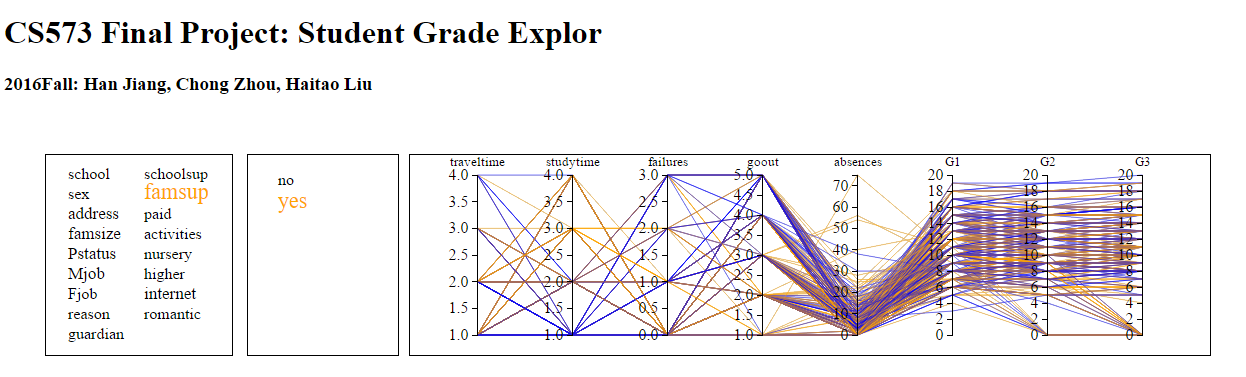
\includegraphics[scale=0.4]{parallel.png}
\caption{On the right side, we use parallel plot to demo the trend of our important features. This plot could interact with users. Users could select part of instance according to some feature values and highlight them. On the left, users could check the feature names and possible feature values.}
\end{figure}
\item [2. Dimension Reduction Projection.]  
The data comes with many features. We project our data into low dimension by PCA, ISOMAP, MDS and TSNE, which people can select by click the button to change the dimension reduction method. \\
Currently, we implement the server side code (server.py). We use python and web.py package to implement the server. When server receive a request from client, it read the server side data, then call dimension reduction function from scikit-learn, then return the dimension reduced data to client as response.\\
\begin{figure}[H]
\centering
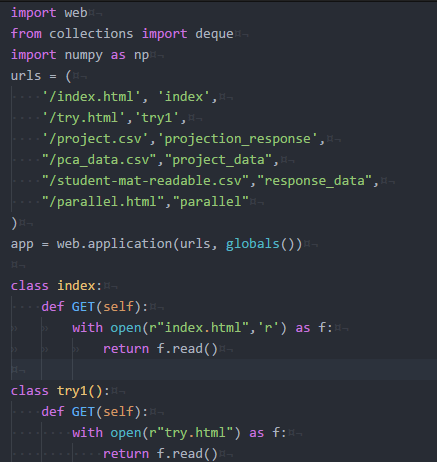
\includegraphics[scale=0.5]{server.png}
\caption{ Implementing a server through web.py is easy. We first build a map matching the url request to its handler class. Web.py puts this mapping in a global tuple variable. Then, we implement every handler class, define a ``Get'' method to response get request. Each ``Get'' method will return the requested file.}
\end{figure}
\end{description}
\section{Reference}
\begin{itemize}
\item UCI data repo Link: {http://archive.ics.uci.edu/ml/datasets/Student+Performance}
\item  USING DATA MINING TO PREDICT SECONDARY SCHOOL STUDENT PERFORMANCE Link: {http://citeseerx.ist.psu.edu/viewdoc/download?doi=10.1.1.540.8151\&rep=rep1\&type=pdf}
\end{itemize}
\end{document}